\documentclass[11pt,a4paper]{article}

\usepackage[a4paper,margin=1in]{geometry}
\usepackage[T1]{fontenc}
\usepackage[utf8]{inputenc}
\usepackage{amsmath}
\usepackage{array}
\usepackage{booktabs}
\usepackage{enumitem}
\usepackage{graphicx}
\usepackage{hyperref}
\usepackage{longtable}
\usepackage{xcolor}
\usepackage{listings}
\usepackage{tikz}

\usetikzlibrary{arrows.meta,positioning,shapes.geometric,fit}

\hypersetup{
  colorlinks=true,
  linkcolor=blue,
  urlcolor=blue,
  pdftitle={TCO Repatriation Dashboard Technical Documentation},
  pdfauthor={TCO Repatriation Dashboard}
}

\lstset{
  basicstyle=\ttfamily\small,
  breaklines=true,
  columns=fullflexible,
  frame=single,
  rulecolor=\color{black!20},
  backgroundcolor=\color{black!3}
}

\setlist[itemize]{leftmargin=*,itemsep=0.2em}
\setlist[enumerate]{leftmargin=*,itemsep=0.2em}
\renewcommand{\arraystretch}{1.18}

\tikzset{
  appbox/.style={rectangle,rounded corners,draw=black!60,fill=blue!6,minimum height=1cm,align=center,text width=3.4cm},
  domainbox/.style={rectangle,rounded corners,draw=black!60,fill=green!7,minimum height=1cm,align=center,text width=3.5cm},
  outbox/.style={rectangle,rounded corners,draw=black!60,fill=orange!10,minimum height=1cm,align=center,text width=3.3cm},
  decision/.style={diamond,draw=black!60,fill=yellow!12,aspect=2,align=center,text width=3.1cm,inner sep=1pt},
  arrow/.style={-{Latex[length=3mm]},thick,draw=black!65}
}

\title{TCO Repatriation Dashboard\\Technical Documentation}
\author{Streamlit application for cloud vs local infrastructure TCO analysis}
\date{May 30, 2026}

\begin{document}

\maketitle
\tableofcontents
\newpage

\section{System Summary}

The TCO Repatriation Dashboard is a local Streamlit application that compares public cloud operating cost against local infrastructure subscription cost over a configurable projection window. It calculates total cost of ownership, savings, break-even timing, monthly run-rate delta, and a rule-based workload placement recommendation.

The project is intentionally small: a Streamlit UI orchestrates a few testable Python modules under \texttt{src/tco}. There is no database, authentication layer, background worker, or external cloud API integration.

\subsection{Core Features}

\begin{itemize}
  \item Manual cloud and local infrastructure cost inputs.
  \item Built-in demo scenarios.
  \item 12 to 60 month projection window.
  \item Public cloud TCO, local infrastructure TCO, savings, and savings percentage.
  \item Break-even month detection.
  \item Rule-based recommendation: cloud-first, hybrid, repatriation, or validate assumptions.
  \item Overview, recommendation, assumptions, monthly detail, and report notes tabs.
  \item CSV export of the monthly projection.
\end{itemize}

\section{Architecture}

\subsection{High-Level Architecture}

The application is a modular monolith. The UI and runtime live in \texttt{app.py}; calculation, recommendation, models, presets, and exports live in separate Python modules.

\begin{center}
\resizebox{0.96\textwidth}{!}{%
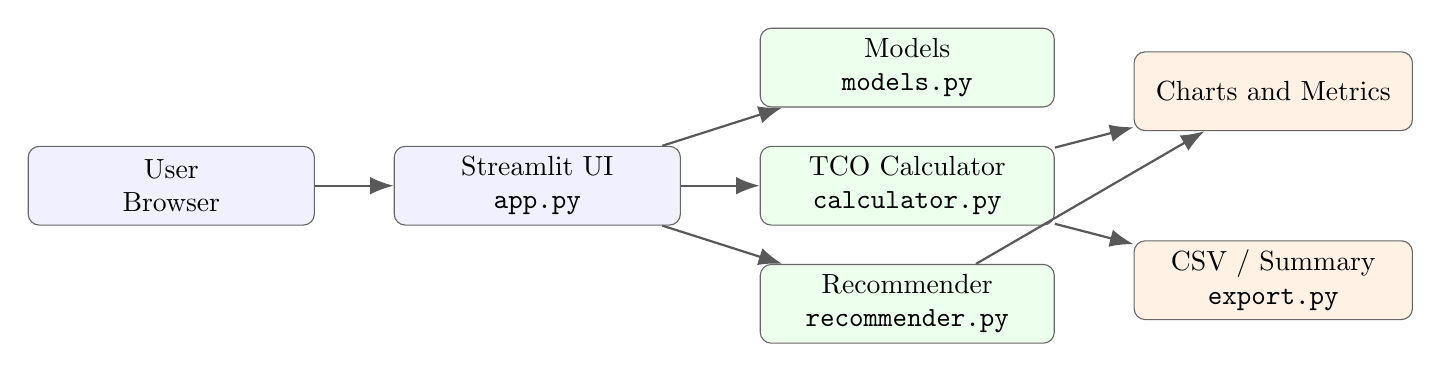
\begin{tikzpicture}[node distance=1.0cm and 1.0cm]
  \node[appbox] (user) {User\\Browser};
  \node[appbox,right=of user] (streamlit) {Streamlit UI\\\texttt{app.py}};
  \node[domainbox,right=of streamlit,yshift=1.5cm] (models) {Models\\\texttt{models.py}};
  \node[domainbox,right=of streamlit] (calc) {TCO Calculator\\\texttt{calculator.py}};
  \node[domainbox,right=of streamlit,yshift=-1.5cm] (reco) {Recommender\\\texttt{recommender.py}};
  \node[outbox,right=of calc,yshift=1.2cm] (charts) {Charts and Metrics};
  \node[outbox,right=of calc,yshift=-1.2cm] (export) {CSV / Summary\\\texttt{export.py}};

  \draw[arrow] (user) -- (streamlit);
  \draw[arrow] (streamlit) -- (models);
  \draw[arrow] (streamlit) -- (calc);
  \draw[arrow] (streamlit) -- (reco);
  \draw[arrow] (calc) -- (charts);
  \draw[arrow] (calc) -- (export);
  \draw[arrow] (reco) -- (charts);
\end{tikzpicture}
}
\end{center}

\subsection{Runtime Flow}

\begin{center}
\resizebox{0.92\textwidth}{!}{%
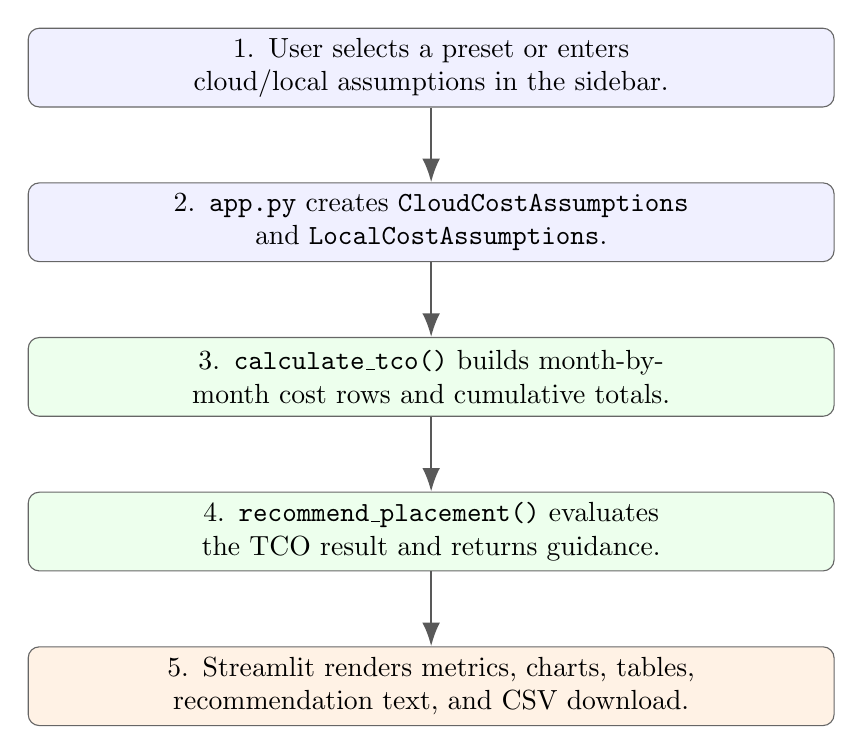
\begin{tikzpicture}[node distance=0.95cm]
  \node[appbox,text width=10cm] (s1) {1. User selects a preset or enters cloud/local assumptions in the sidebar.};
  \node[appbox,text width=10cm,below=of s1] (s2) {2. \texttt{app.py} creates \texttt{CloudCostAssumptions} and \texttt{LocalCostAssumptions}.};
  \node[domainbox,text width=10cm,below=of s2] (s3) {3. \texttt{calculate\_tco()} builds month-by-month cost rows and cumulative totals.};
  \node[domainbox,text width=10cm,below=of s3] (s4) {4. \texttt{recommend\_placement()} evaluates the TCO result and returns guidance.};
  \node[outbox,text width=10cm,below=of s4] (s5) {5. Streamlit renders metrics, charts, tables, recommendation text, and CSV download.};

  \draw[arrow] (s1) -- (s2);
  \draw[arrow] (s2) -- (s3);
  \draw[arrow] (s3) -- (s4);
  \draw[arrow] (s4) -- (s5);
\end{tikzpicture}
}
\end{center}

\subsection{Layer Responsibilities}

\begin{longtable}{p{0.28\textwidth}p{0.34\textwidth}p{0.28\textwidth}}
\toprule
\textbf{Layer} & \textbf{Files} & \textbf{Responsibility} \\
\midrule
Presentation & \texttt{app.py} & Streamlit page, sidebar inputs, tabs, charts, and formatting. \\
Domain models & \texttt{src/tco/models.py} & Dataclasses and validation for assumptions and results. \\
Calculation & \texttt{src/tco/calculator.py} & Projection, growth, cumulative totals, and break-even logic. \\
Recommendation & \texttt{src/tco/recommender.py} & Rule-based workload placement recommendation. \\
Presets & \texttt{src/tco/presets.py} & Built-in demo scenarios. \\
Export & \texttt{src/tco/export.py} & CSV projection and executive summary text. \\
Tests & \texttt{tests/} & Formula, break-even, discount, and recommendation path tests. \\
\bottomrule
\end{longtable}

\section{Data Model}

\subsection{Model Relationships}

\begin{center}
\resizebox{0.96\textwidth}{!}{%
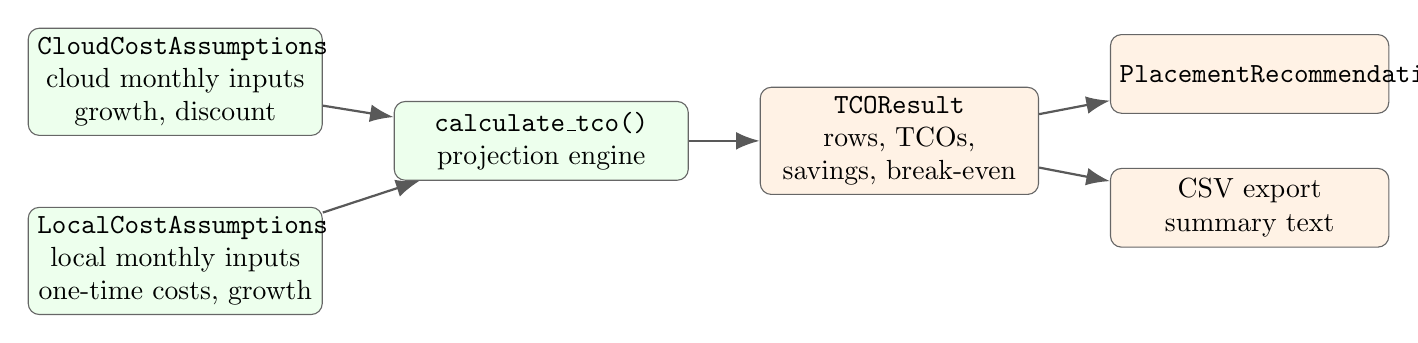
\begin{tikzpicture}[node distance=0.9cm and 0.9cm]
  \node[domainbox] (cloud) {\texttt{CloudCostAssumptions}\\cloud monthly inputs\\growth, discount};
  \node[domainbox,below=of cloud] (local) {\texttt{LocalCostAssumptions}\\local monthly inputs\\one-time costs, growth};
  \node[domainbox,right=of cloud,yshift=-0.75cm] (calc) {\texttt{calculate\_tco()}\\projection engine};
  \node[outbox,right=of calc] (result) {\texttt{TCOResult}\\rows, TCOs, savings, break-even};
  \node[outbox,right=of result,yshift=0.85cm] (reco) {\texttt{PlacementRecommendation}};
  \node[outbox,right=of result,yshift=-0.85cm] (csv) {CSV export\\summary text};

  \draw[arrow] (cloud) -- (calc);
  \draw[arrow] (local) -- (calc);
  \draw[arrow] (calc) -- (result);
  \draw[arrow] (result) -- (reco);
  \draw[arrow] (result) -- (csv);
\end{tikzpicture}
}
\end{center}

\subsection{Key Dataclasses}

\begin{longtable}{p{0.32\textwidth}p{0.58\textwidth}}
\toprule
\textbf{Dataclass} & \textbf{Purpose} \\
\midrule
\texttt{CloudCostAssumptions} & Cloud monthly line items, annual growth rate, and discount. \\
\texttt{LocalCostAssumptions} & Local monthly line items, annual growth rate, migration cost, and installation cost. \\
\texttt{ProjectionRow} & One projected month containing monthly and cumulative cloud/local costs. \\
\texttt{TCOResult} & Full projection output and derived metrics. \\
\texttt{PlacementRecommendation} & Recommendation label, confidence, headline, rationale, and next-step guidance. \\
\bottomrule
\end{longtable}

\section{Calculation Logic}

\subsection{Projection Window}

The default projection is 36 months. The UI supports 12 to 60 months.

\subsection{Growth Multiplier}

For month \(m\), the growth multiplier is:

\[
\text{growth\_multiplier}(m) = \left(1 + \frac{\text{annual\_growth\_rate\_pct}}{100}\right)^{\frac{m - 1}{12}}
\]

Month 1 uses multiplier \(1.0\).

\subsection{Cloud Monthly Baseline}

\[
\text{cloud\_base} = \text{compute} + \text{storage} + \text{database} + \text{network} + \text{backup} + \text{support}
\]

\[
\text{cloud\_after\_discount} = \text{cloud\_base} \times \left(1 - \frac{\text{discount\_pct}}{100}\right)
\]

\[
\text{cloud\_month}_m = \text{cloud\_after\_discount} \times \text{growth\_multiplier}(m)
\]

\subsection{Local Monthly Baseline}

\[
\begin{aligned}
\text{local\_base} ={}& \text{infrastructure\_subscription} + \text{software\_licenses} + \text{support\_contract} \\
& + \text{power\_cooling} + \text{datacenter} + \text{admin\_labor} + \text{backup\_dr}
\end{aligned}
\]

\[
\text{local\_month}_m = \text{local\_base} \times \text{growth\_multiplier}(m)
\]

\subsection{One-Time Local Cost}

\[
\text{one\_time\_local} = \text{migration\_one\_time} + \text{installation\_one\_time}
\]

This amount is included before local monthly costs accumulate.

\subsection{TCO, Savings, And Break-Even}

\[
\text{cloud\_tco} = \sum_{m=1}^{n} \text{cloud\_month}_m
\]

\[
\text{local\_tco} = \text{one\_time\_local} + \sum_{m=1}^{n} \text{local\_month}_m
\]

\[
\text{savings} = \text{cloud\_tco} - \text{local\_tco}
\]

\[
\text{savings\_pct} = \frac{\text{savings}}{\text{cloud\_tco}} \times 100
\]

Break-even is the first month where:

\[
\text{local\_cumulative} \leq \text{cloud\_cumulative}
\]

If this condition is never reached inside the projection window, break-even is reported as not reached.

\section{Recommendation Logic}

\subsection{Recommendation Inputs}

The recommender uses only the computed TCO result and cloud cost distribution:

\begin{itemize}
  \item Cloud TCO.
  \item Local TCO.
  \item Savings percentage.
  \item Break-even month.
  \item Monthly run-rate delta.
  \item Dominant cloud cost category.
  \item Cloud discount percentage.
\end{itemize}

\subsection{Decision Tree}

\begin{center}
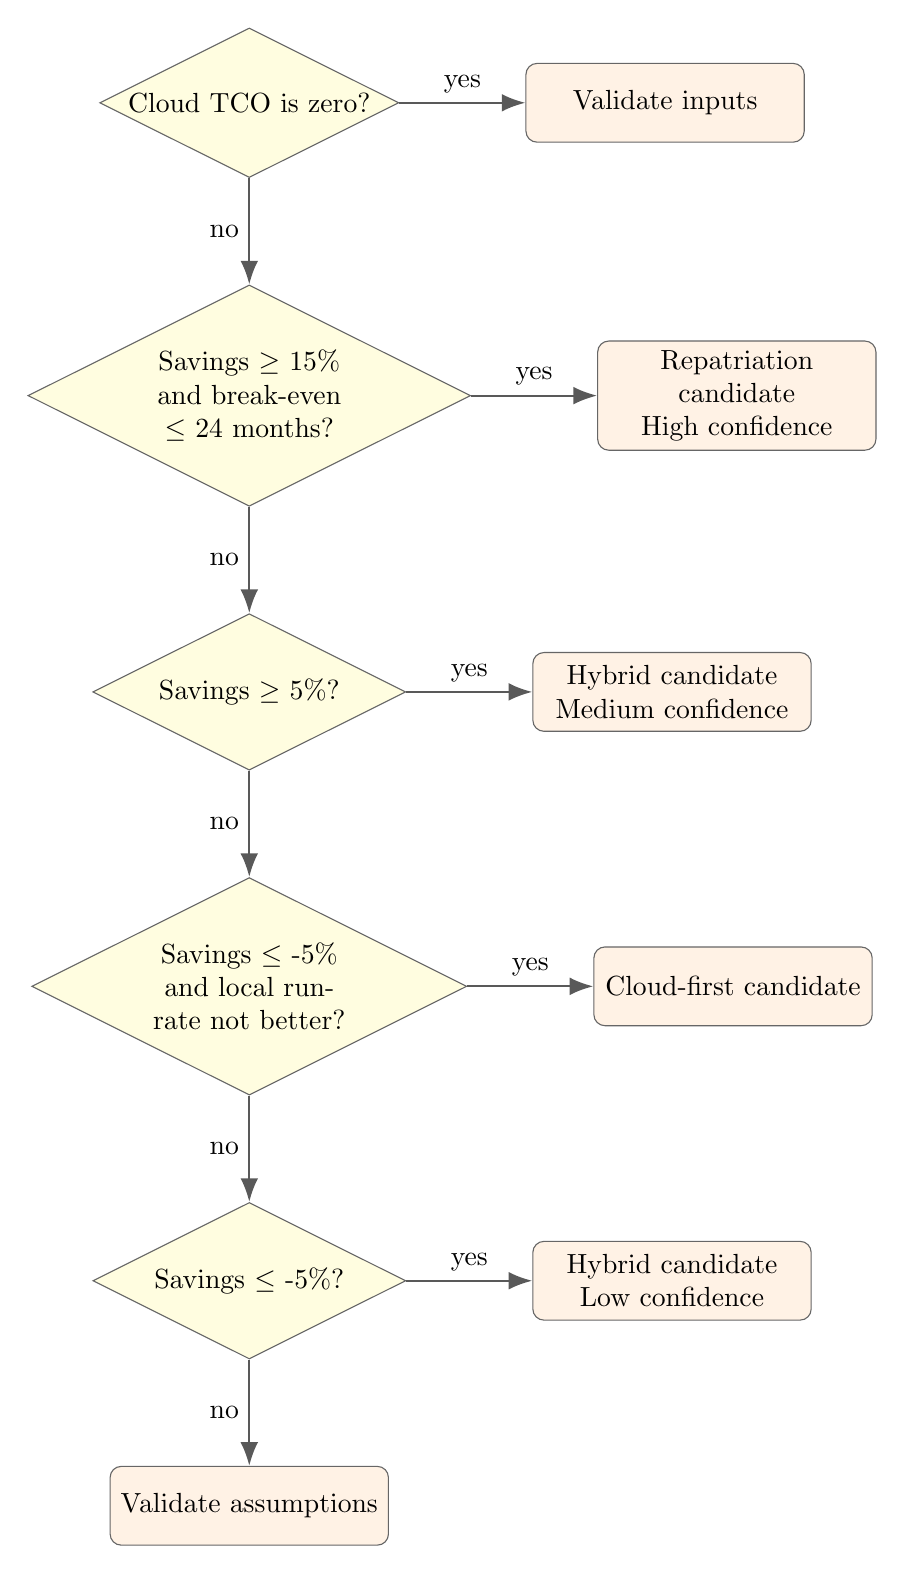
\begin{tikzpicture}[node distance=1.35cm and 1.6cm]
  \node[decision] (a) {Cloud TCO is zero?};
  \node[outbox,right=of a] (invalid) {Validate inputs};
  \node[decision,below=of a] (b) {Savings \(\geq\) 15\% and break-even \(\leq\) 24 months?};
  \node[outbox,right=of b] (rep) {Repatriation candidate\\High confidence};
  \node[decision,below=of b] (c) {Savings \(\geq\) 5\%?};
  \node[outbox,right=of c] (hyb) {Hybrid candidate\\Medium confidence};
  \node[decision,below=of c] (d) {Savings \(\leq\) -5\% and local run-rate not better?};
  \node[outbox,right=of d] (cloudfirst) {Cloud-first candidate};
  \node[decision,below=of d] (e) {Savings \(\leq\) -5\%?};
  \node[outbox,right=of e] (hyblow) {Hybrid candidate\\Low confidence};
  \node[outbox,below=of e] (validate) {Validate assumptions};

  \draw[arrow] (a) -- node[above] {yes} (invalid);
  \draw[arrow] (a) -- node[left] {no} (b);
  \draw[arrow] (b) -- node[above] {yes} (rep);
  \draw[arrow] (b) -- node[left] {no} (c);
  \draw[arrow] (c) -- node[above] {yes} (hyb);
  \draw[arrow] (c) -- node[left] {no} (d);
  \draw[arrow] (d) -- node[above] {yes} (cloudfirst);
  \draw[arrow] (d) -- node[left] {no} (e);
  \draw[arrow] (e) -- node[above] {yes} (hyblow);
  \draw[arrow] (e) -- node[left] {no} (validate);
\end{tikzpicture}
\end{center}

\subsection{Dominant Category Adjustment}

If one public cloud category is at least 35 percent of cloud baseline spend, the recommendation adds context:

\begin{itemize}
  \item Storage or backup dominant: prioritize storage-heavy or backup-heavy workloads for local evaluation, unless cloud-first is already recommended.
  \item Compute dominant with at least 10 percent cloud discount: keep bursty or elastic compute cloud-side unless utilization is consistently high.
  \item Database dominant and not a repatriation case: keep managed databases in cloud unless operations ownership is clearly covered.
\end{itemize}

\section{User Interface}

\subsection{Sidebar}

The sidebar collects all scenario inputs:

\begin{itemize}
  \item Scenario preset, apply preset action, scenario name, and projection window.
  \item Cloud line items: compute, storage, database, network, backup, support, annual growth, and discount.
  \item Local line items: infrastructure subscription, software licenses, support contract, power/cooling, datacenter, admin labor, backup/DR, annual growth, migration cost, and installation cost.
\end{itemize}

\subsection{Tabs}

\begin{longtable}{p{0.25\textwidth}p{0.65\textwidth}}
\toprule
\textbf{Tab} & \textbf{Purpose} \\
\midrule
Overview & Shows headline TCO metrics, savings, break-even, summary, and charts. \\
Recommendation & Shows placement label, confidence, rationale, and first actions. \\
Assumptions & Shows the cost inputs used by the model. \\
Monthly Detail & Shows every projected month and cumulative cost values. \\
Report Notes & Summarizes the result for a simple presales or review note. \\
\bottomrule
\end{longtable}

\section{Repository Structure}

\begin{lstlisting}
app.py
src/tco/
  __init__.py
  calculator.py
  export.py
  models.py
  presets.py
  recommender.py
tests/
  __init__.py
  test_calculator.py
  test_recommender.py
docs/
  *.md
.streamlit/
  config.toml
\end{lstlisting}

\section{Setup And Execution}

\subsection{Install Dependencies}

\begin{lstlisting}
python -m venv .venv
.\.venv\Scripts\Activate.ps1
pip install -r requirements.txt
\end{lstlisting}

\subsection{Run The App}

\begin{lstlisting}
streamlit run app.py --server.port 8502
\end{lstlisting}

Open:

\begin{lstlisting}
http://localhost:8502
\end{lstlisting}

\subsection{Run Tests}

\begin{lstlisting}
python -m unittest discover
python -m pytest
python -m compileall app.py src tests
\end{lstlisting}

\section{Testing Scope}

\begin{longtable}{p{0.36\textwidth}p{0.54\textwidth}}
\toprule
\textbf{Test File} & \textbf{Coverage} \\
\midrule
\texttt{tests/test\_calculator.py} & Projection totals, break-even behavior, cloud discount, and case where local is always more expensive. \\
\texttt{tests/test\_recommender.py} & Main recommendation paths: repatriation, hybrid, cloud-first, and validate assumptions. \\
\bottomrule
\end{longtable}

Manual verification should confirm that presets apply, sidebar inputs load, charts render, recommendation output appears, monthly detail renders, assumptions match inputs, and CSV export works.

\section{Operational Notes}

\subsection{Known Constraints}

\begin{itemize}
  \item No cloud billing import.
  \item No database or saved scenarios.
  \item No authentication.
  \item No PDF report export.
  \item No NPV, depreciation, tax, or workload-sizing model.
  \item Recommendation is rule-based and depends entirely on entered assumptions.
\end{itemize}

\subsection{Common Issues}

\begin{longtable}{p{0.32\textwidth}p{0.58\textwidth}}
\toprule
\textbf{Issue} & \textbf{Fix} \\
\midrule
\texttt{ModuleNotFoundError: streamlit} & Run \texttt{pip install -r requirements.txt}. \\
Port \texttt{8502} in use & Run on another port, for example \texttt{--server.port 8503}. \\
Tests do not discover & Run \texttt{python -m unittest discover -s tests -p "test\_*.py"}. \\
Theme looks wrong & Check \texttt{.streamlit/config.toml}; the expected base theme is light. \\
Unexpected recommendation & Review savings percentage, break-even, monthly run-rate delta, cloud discount, and dominant cloud cost category. \\
\bottomrule
\end{longtable}

\section{Future Improvements}

The most natural next improvements are:

\begin{itemize}
  \item PDF executive report export.
  \item Saved scenario comparison.
  \item Optional billing CSV import.
  \item Discovery checklist mapped to sidebar inputs.
  \item More tests for exports, presets, zero-cost cases, and chart helpers.
\end{itemize}

\end{document}
